\item O tronco de cone é formado girando-se a área sombreada em torno do eixo $x$. Determine o momento de inércia $I$, e expresse o resultado em termos da massa total $m$ do tronco. O tronco tem uma densidade constante $\rho$.

\vspace{-.7cm}
\begin{flushright}
	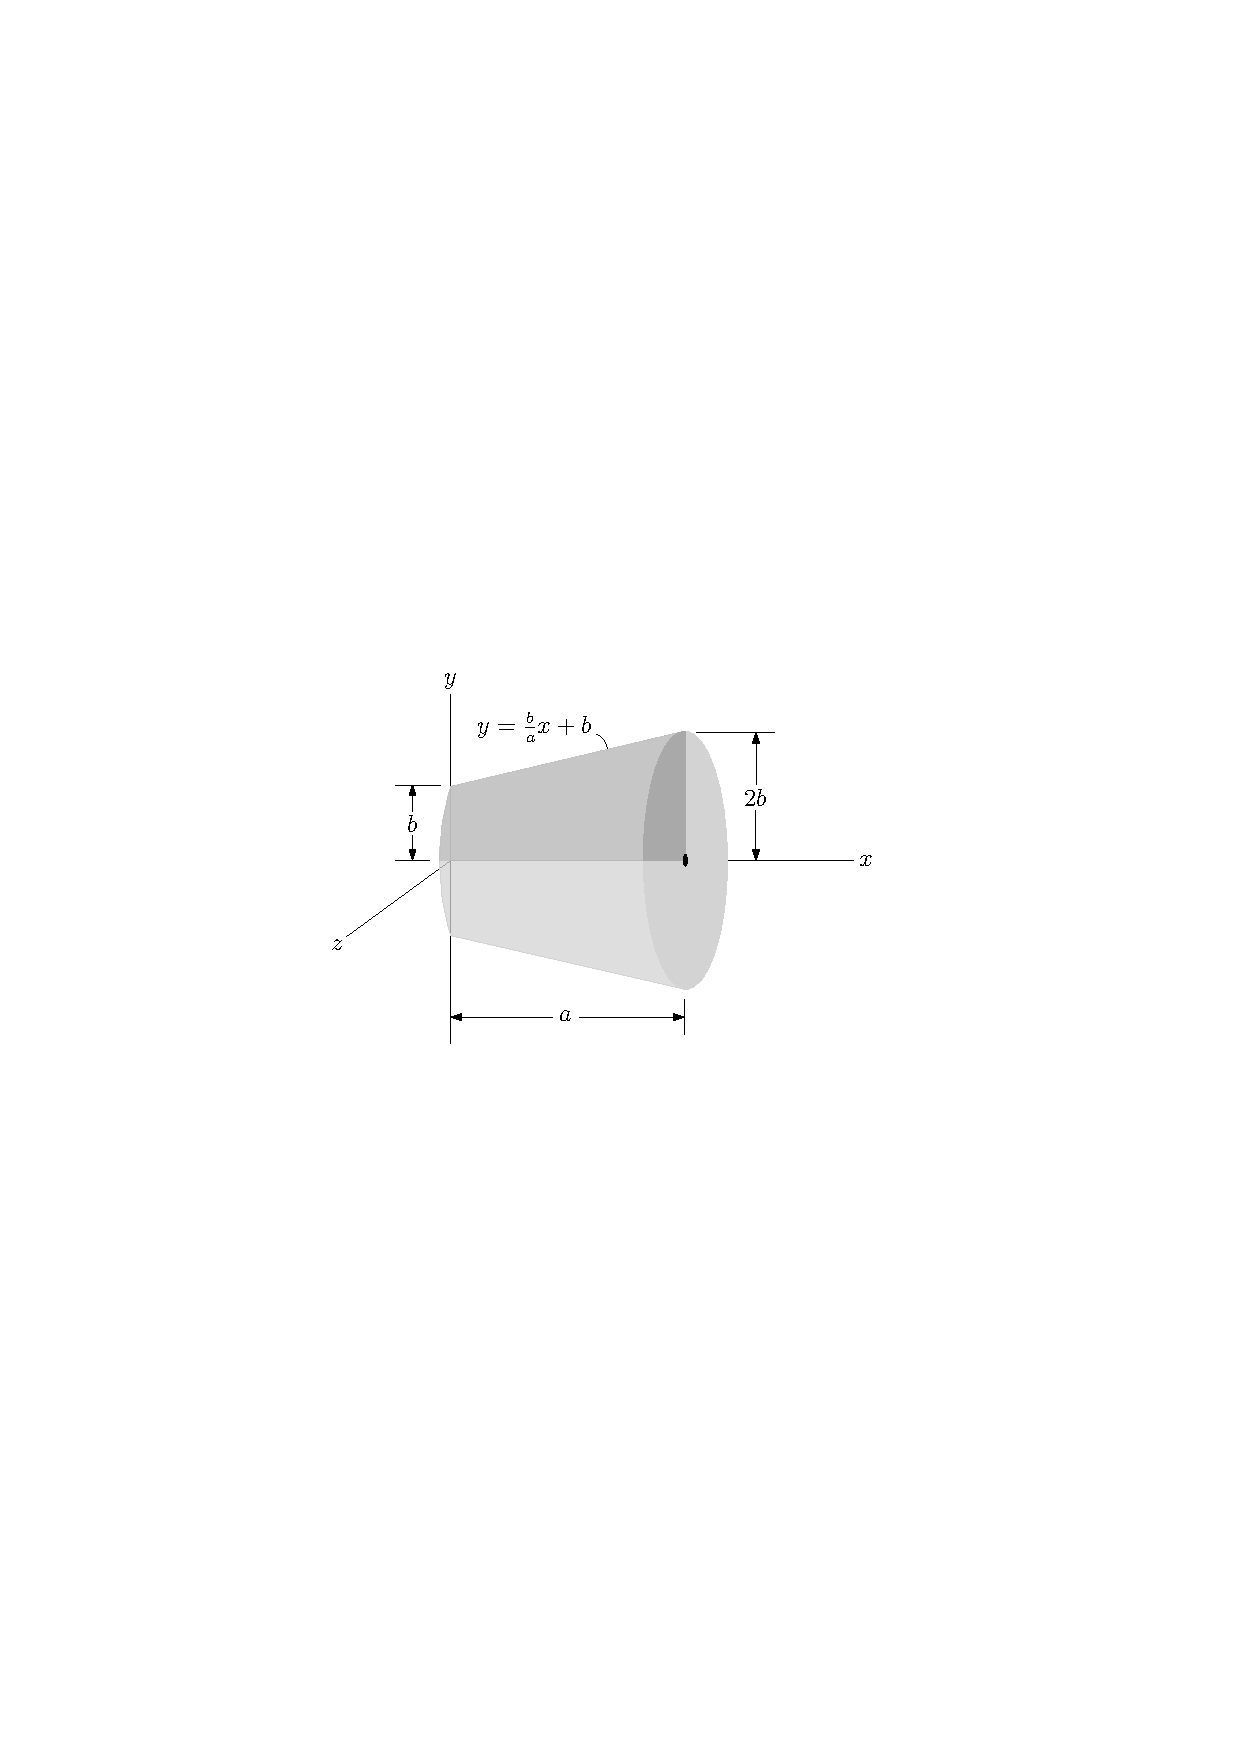
\includegraphics[scale=1.05]{../../images/draw_1}
\end{flushright}